\chapter{Activities \& Interaction}

\section{Aims}
\paragraph{} At the end of the practical portion of this topic you will be able to:

\begin{itemize}
\item Work with Android Activities
\item Work with user input views
\end{itemize}

\section{Activities}
\paragraph{} We will start the lab by working with activities. The Android project defines an Activity as a ``single, focused thing that the user can do''. This can mean quite a few things but for out purposes at this stage we will consider an activity as essentially a single screen of an Android app that probably contains some user interface elements to enable interaction. An app can have zero or more activities, but usually we will be dealing with at least one activity. When we go through the wizard to create a new Android project, a single default empty activity is created for us, and, in the previous chapters, we have added things to this activity, like buttons for user interaction, but we haven't moved to a different screen, that is we haven't switched to a different activity (mainly because we only have the one available to us). In HelloAndroid we got a single activity by default that we used to display some views. However, using multiple activities and switching between them can be a useful way to organise your app if you want your user to navigate between multiple screens. So in this part of the lab we will look at creating activities, displaying them, and navigating between them.

\subsection{What do we have?}
\paragraph{} When we create an Android Activity with an empty activity\footnote{If you're on an older version of Android studio or using an older API level or SDK then this might be referred to as a ``Blank'' Activity. These are essentially the same. Note however that if you choose a ``Basic'' Activity then extra code that you might not necessarily use will be generated for you.} we get some code generated for us. There are some things to be aware of here:

\begin{itemize}
\item The empty activity created by the wizard contains a Java file and an XML file. The XML file describes the ``view'', the way that the screen made visible to the user should look. The Java file then contains code to actually perform tasks related to that view. For example, if your view, that is your XML file, contains a description for a  button, then your Java file must contain some code that does something when the button is clicked. Of course the Java file can contain code that does much more, pretty much anything that you can do in the Java language, but let's keep things simple for now, or at least as simple as the Android platform will allow us. An entire, default, boilerplate AppCompatActivity Java file looks like this:

\begin{lstlisting}

package org.simonwells.testapp;

import android.support.v7.app.AppCompatActivity;
import android.os.Bundle;

public class MainActivity extends AppCompatActivity {

    @Override
    protected void onCreate(Bundle savedInstanceState) {
        super.onCreate(savedInstanceState);
        setContentView(R.layout.activity_main);
    }
}
\end{lstlisting}

and the corresponding XML file for the default, corresponding layout looks like this:

\begin{lstlisting}
<?xml version="1.0" encoding="utf-8"?>
<RelativeLayout xmlns:android="http://schemas.android.com/apk/res/android"
    xmlns:tools="http://schemas.android.com/tools"
    android:id="@+id/activity_main"
    android:layout_width="match_parent"
    android:layout_height="match_parent"
    android:paddingBottom="@dimen/activity_vertical_margin"
    android:paddingLeft="@dimen/activity_horizontal_margin"
    android:paddingRight="@dimen/activity_horizontal_margin"
    android:paddingTop="@dimen/activity_vertical_margin"
    tools:context="org.simonwells.testapp.MainActivity">

    <TextView
        android:layout_width="wrap_content"
        android:layout_height="wrap_content"
        android:text="Hello World!" />
</RelativeLayout>
\end{lstlisting}



\item Generally an Empty Activity will contain a Java class that \emph{inherits} from the Activity base class. This is a technical term from object oriented programming that means that we have taken a basic \emph{template} for some code, then added some new stuff to the template to create a child and that the child gets all the code from the parent plus the new added code that make it into a child. Note however that in our Java file it says

\begin{lstlisting}
    public class MainActivity extends AppCompatActivity {
\end{lstlisting}

This means that our specific Activity is a child of the Activity base class and our child class is called AppCompatActivity. This is an Activity that adds extra features to the base class to support different functionality. In this specific case, AppCompatActivity adds support for the Action Bar. The Action bar is that part of an Android app at the top of the screen that usually holds buttons and important actions that you need throughout your app. The Action Bar usually includes some, but not necessarily all of the following: an App Icon, a control for changing the view, action buttons for the most important interactions with your app, and an overflow menu for further, less frequently used actions.

\item There are many different activities available. For the most part we will only use the Empty (or Blank) Activity initially. Although during your coursework you might choose to use other Activities in your implementation, but that is a design decision for you to make. That said, there are also ``Basic'' Activities, which support Fragments,a way to organise your screen into smaller logical parts so that you can more easily control how your app's widgets are displayed and organised across different devices, ``Fullscreen'' Activities, useful if you want to use every part of the device's display, and other Activities that are pre-filled with skeleton code to do specific tasks. For example, there are Activities that support Google Maps integration, use of navigation drawers, and many other things. Investigate the various Activities and compare the differences between them. The easiest way to do this is to create new Android Studio projects and select different Activities from the ``Add Activity'' page of the wizard. Mostly you will find that the different types of Activity are just Activities, i.e. they inherit from the Activity base class\footnote{The JavaDoc for the Activity base class is here: \url{https://developer.android.com/reference/android/app/Activity.html}. You should read through this page to better understand the technical aspects of Activities}. 
\end{itemize}


\subsection{Creating New Activities}
\paragraph{} Most of the Android apps that we use probably have more than one screen. Think of all of the apps that you have used and the number of different screens that you might navigate through in order to perform different tasks. At the very least, even the simplest app, where you can do most things from a single screen, usually have a second screen to allow you to adjust your settings and personal preferences. If an app has more than one screen then it will also have more than one activity. More than one activity basically means more than one java file containing a class that inherits from Activity, and more than one layout file to give a view, or screen, for the Activity. This means that if we want to have more than one Activity in our Android apps then we are going to have to add new Java and XML files. There are two ways to do this, the easy way, which you will probably use most often, which involves letting Android Studio add the new file that you dictate. The alternative is to manually add the Java and XML files into the project. We can try both, and it is a good idea to do both at least once, but generally the easiest method is to let Android Studio do all the work and produce the correct files.

\subsubsection{Adding a new Activity}
\paragraph{} Creating new activities is straightforward if you are working in Android Studio as it provides helper wizards to add the new code for you. For example, if in the studio interface you right click on the app folder in the project explorer then select ``New'' $>$ ``Activity'' $>$ ``Empty Activity'' and accept the defaults then Android Studio will add in the necessary code to support your new Activity.

\begin{figure}[H]
\centering
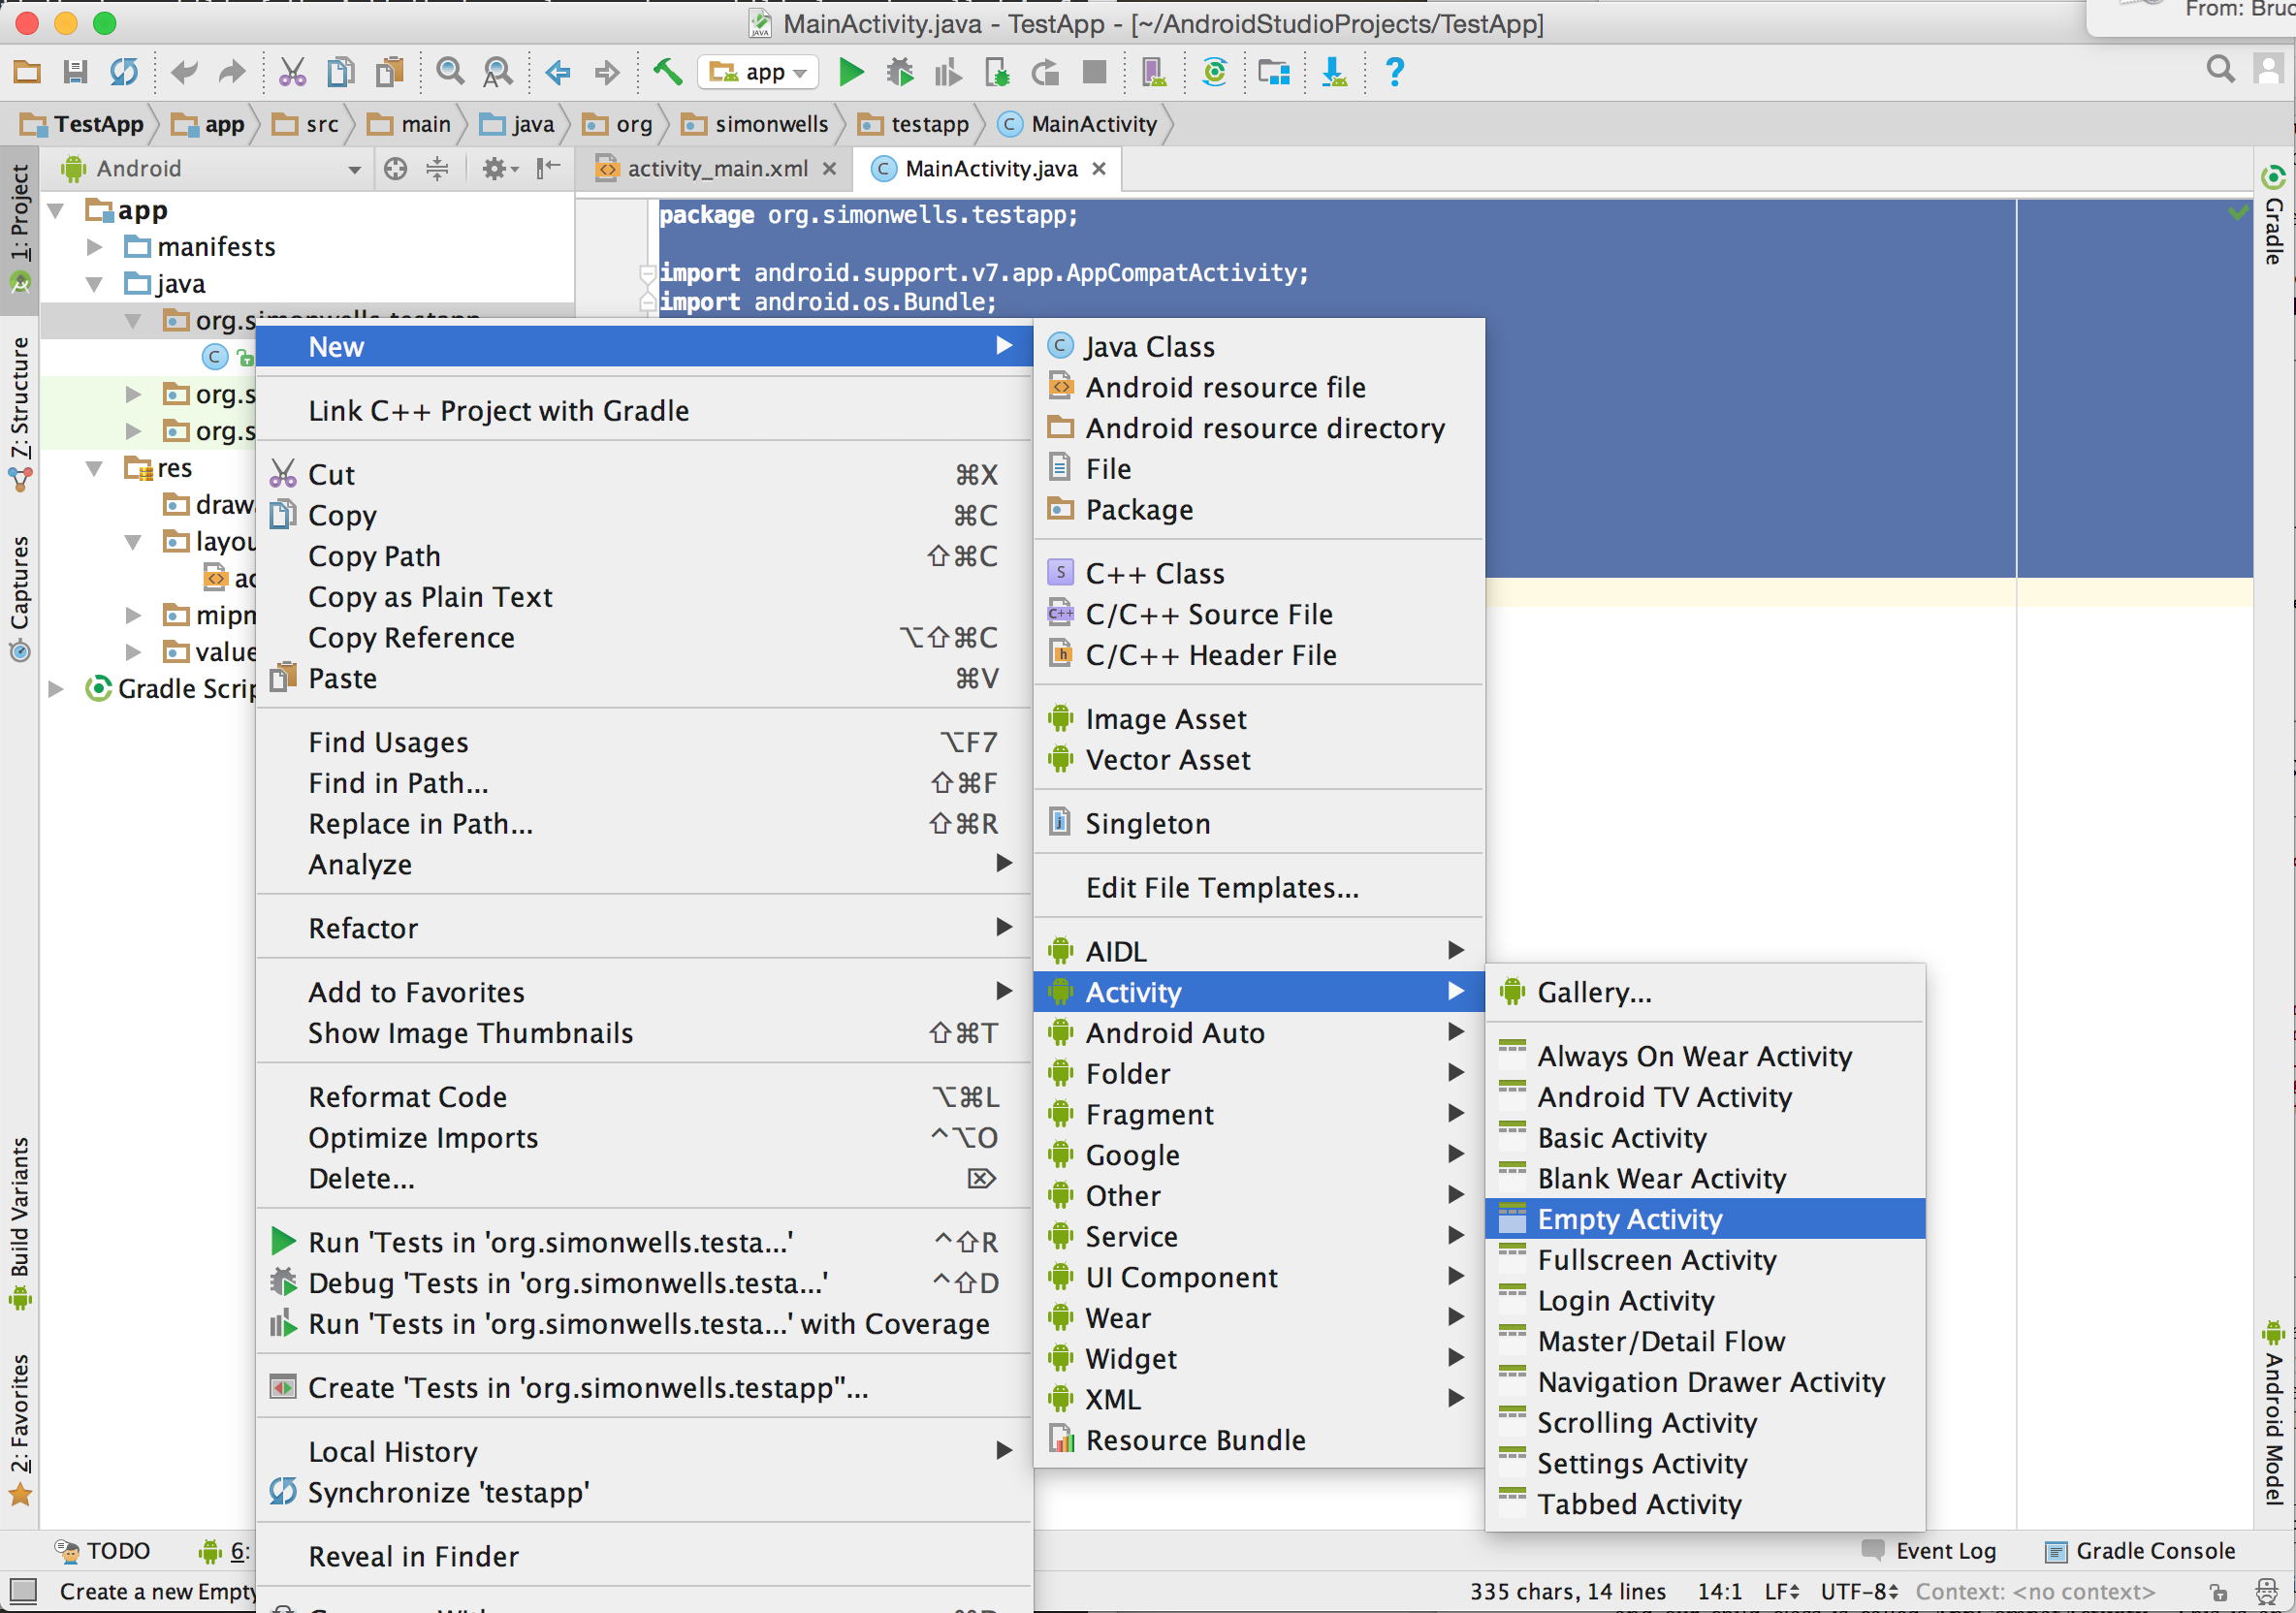
\includegraphics[width=\textwidth]{images/activities_add_activity_studio}
\caption{Android Studio Add Activity Options}
\label{fig:activities_add_activity_studio}
\end{figure}


\paragraph{} The new files that are generated for you include a java src file called `Main2Activity.java', an XML activity file called `activity\_main2.xml', and an entry in the AndroidManifest.xml file. Our project layout should now look something like the following:

\begin{figure}[H]
\centering
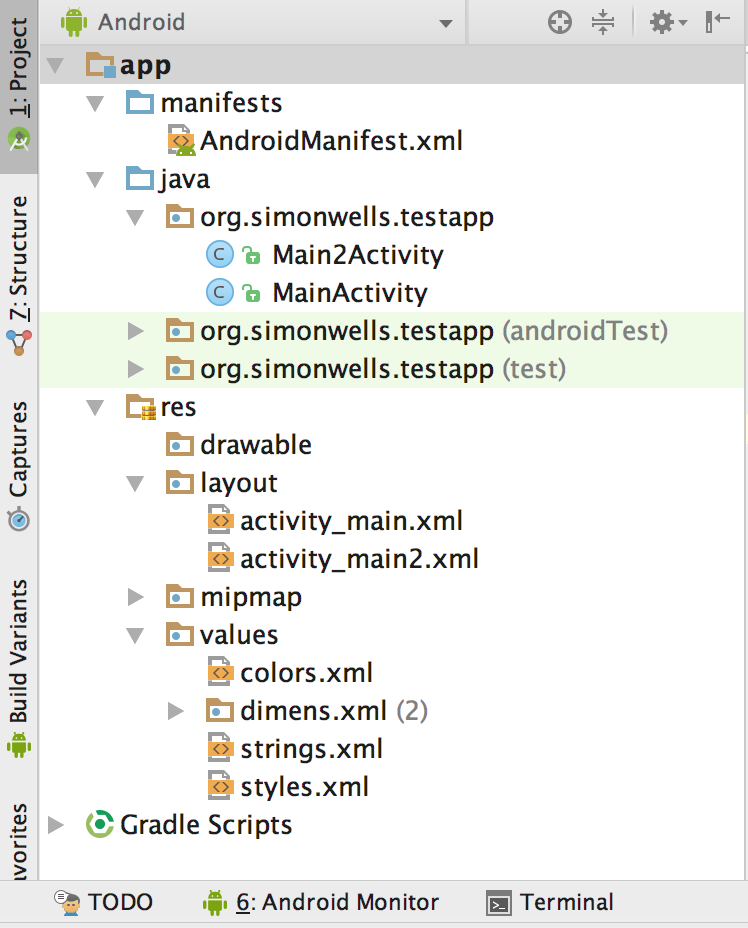
\includegraphics[width=\textwidth]{images/activities_project_explorer}
\caption{Android Project Files}
\label{fig:activities_project_explorer}
\end{figure}

\paragraph{} Notice that we have new Java and resource files for our new activity. Open up these files and explore tham. Compare the new activity files to the ones we started with. Other than different names, there should not be too much difference between them.

\paragraph{} There shouldn't be any real surprises in the MainActivity2.java file but if you are unsure, compare it to MainActivity.java

\begin{lstlisting}
package org.simonwells.testapp;

import android.support.v7.app.AppCompatActivity;
import android.os.Bundle;

public class Main2Activity extends AppCompatActivity {

    @Override
    protected void onCreate(Bundle savedInstanceState) {
        super.onCreate(savedInstanceState);
        setContentView(R.layout.activity_main2);
    }
}
\end{lstlisting}

\paragraph{} The layout for activity\_main2.xml looks pretty similar to activity\_main.xml

\begin{lstlisting}
<?xml version="1.0" encoding="utf-8"?>
<RelativeLayout xmlns:android="http://schemas.android.com/apk/res/android"
    xmlns:tools="http://schemas.android.com/tools"
    android:id="@+id/activity_main2"
    android:layout_width="match_parent"
    android:layout_height="match_parent"
    android:paddingBottom="@dimen/activity_vertical_margin"
    android:paddingLeft="@dimen/activity_horizontal_margin"
    android:paddingRight="@dimen/activity_horizontal_margin"
    android:paddingTop="@dimen/activity_vertical_margin"
    tools:context="org.simonwells.testapp.Main2Activity">

</RelativeLayout>

\end{lstlisting}

\paragraph{} As well as generating new files, Android Studio add a Manifest entry for the new Activity as shown here:

\begin{lstlisting}
<?xml version="1.0" encoding="utf-8"?>
<manifest xmlns:android="http://schemas.android.com/apk/res/android"
    package="org.simonwells.testapp">

    <application
        android:allowBackup="true"
        android:icon="@mipmap/ic_launcher"
        android:label="@string/app_name"
        android:supportsRtl="true"
        android:theme="@style/AppTheme">
        <activity android:name=".MainActivity">
            <intent-filter>
                <action android:name="android.intent.action.MAIN" />

                <category android:name="android.intent.category.LAUNCHER" />
            </intent-filter>
        </activity>
        <activity android:name=".Main2Activity"></activity>
    </application>

</manifest>
\end{lstlisting}


\paragraph{} That is all that is needed to create a new Activity as far as Android is concerned. Basically, two new files, a Java source file and an XML layout file, plus a couple of edits to the Android Manifest to make sure that your app knows about the new stuff. You can now run your app.

\paragraph{} Hmmm. Not much difference there? Why do you think that is?

\subsubsection{Switching Activities using the Android Manifest}

\paragraph{} The quickest way to display your new Activity is to edit the AndroidManifest.xml to tell it to launch the new activity instead of the default. Let's do that. All we need to do is move the $<$intent-filter$>$ block from MainActivity to our new MainActivity2 block as follows:
\begin{lstlisting}
<?xml version="1.0" encoding="utf-8"?>
<manifest xmlns:android="http://schemas.android.com/apk/res/android"
    package="org.simonwells.testapp">

    <application
        android:allowBackup="true"
        android:icon="@mipmap/ic_launcher"
        android:label="@string/app_name"
        android:supportsRtl="true"
        android:theme="@style/AppTheme">
        <activity android:name=".MainActivity"></activity>
        <activity android:name=".Main2Activity">
            <intent-filter>
                <action android:name="android.intent.action.MAIN" />

                <category android:name="android.intent.category.LAUNCHER" />
            </intent-filter>
        </activity>
    </application>

</manifest>
\end{lstlisting}


\paragraph{} Now run your app. You should now see the second Activity displayed. You can tell the difference because your second activity doesn't have the hello world message. Try adding some new elements to your Activities so that you can tell them apart more easily.

\paragraph{} But this isn't really good enough. We can't edit the app's manifest file every time we want to create a new Activity. We need another approach.

\subsubsection{Launching a new Activity from code}
\paragraph{} Create a new Android Studio project and add a second activity as we did earlier in the chapter. Once you know that it compiles and runs correctly you can do the following: Add a button to activity\_main.xml then add a handler for the button to your MainActivity.java file so that it looks like the following:

\begin{lstlisting}
package org.simonwells.testapp;

import android.content.Intent;
import android.support.v7.app.AppCompatActivity;
import android.os.Bundle;
import android.view.View;
import android.widget.Button;

public class MainActivity extends AppCompatActivity {

    @Override
    protected void onCreate(Bundle savedInstanceState) {
        super.onCreate(savedInstanceState);
        setContentView(R.layout.activity_main);

        Button btn = (Button) findViewById(R.id.button);
        btn.setOnClickListener(new View.OnClickListener() {
            @Override
            public void onClick(View view) {
                Intent activity2 = new Intent(MainActivity.this, Main2Activity.class);
                startActivity(activity2);
            }
        });
    }
}
\end{lstlisting}

\paragraph{} and your corresponding activity\_main.xml will look like this:

\begin{lstlisting}
<?xml version="1.0" encoding="utf-8"?>
<RelativeLayout xmlns:android="http://schemas.android.com/apk/res/android"
    xmlns:tools="http://schemas.android.com/tools"
    android:id="@+id/activity_main"
    android:layout_width="match_parent"
    android:layout_height="match_parent"
    android:paddingBottom="@dimen/activity_vertical_margin"
    android:paddingLeft="@dimen/activity_horizontal_margin"
    android:paddingRight="@dimen/activity_horizontal_margin"
    android:paddingTop="@dimen/activity_vertical_margin"
    tools:context="org.simonwells.testapp.MainActivity">

    <TextView
        android:layout_width="wrap_content"
        android:layout_height="wrap_content"
        android:text="Hello World!"
        android:id="@+id/textView" />

    <Button
        android:text="Button"
        android:layout_width="wrap_content"
        android:layout_height="wrap_content"
        android:layout_below="@+id/textView"
        android:layout_centerHorizontal="true"
        android:layout_marginTop="170dp"
        android:id="@+id/button" />
</RelativeLayout>

\end{lstlisting}

\paragraph{} Now run your app. You should be able to click the button and cause the second activity to be displayed. You will have to use the device's back button to return to the previous Activity. Consider how you might return to the previous activity from within your app? Perhaps a button or other navigation element that, when clicked finishes the current Activity and returns you to the parent? Do some research and see if you can work out how to do this for yourself.

\begin{figure}[H]%[htb]
\centering
    \begin{subfigure}[b]{0.45\textwidth}
        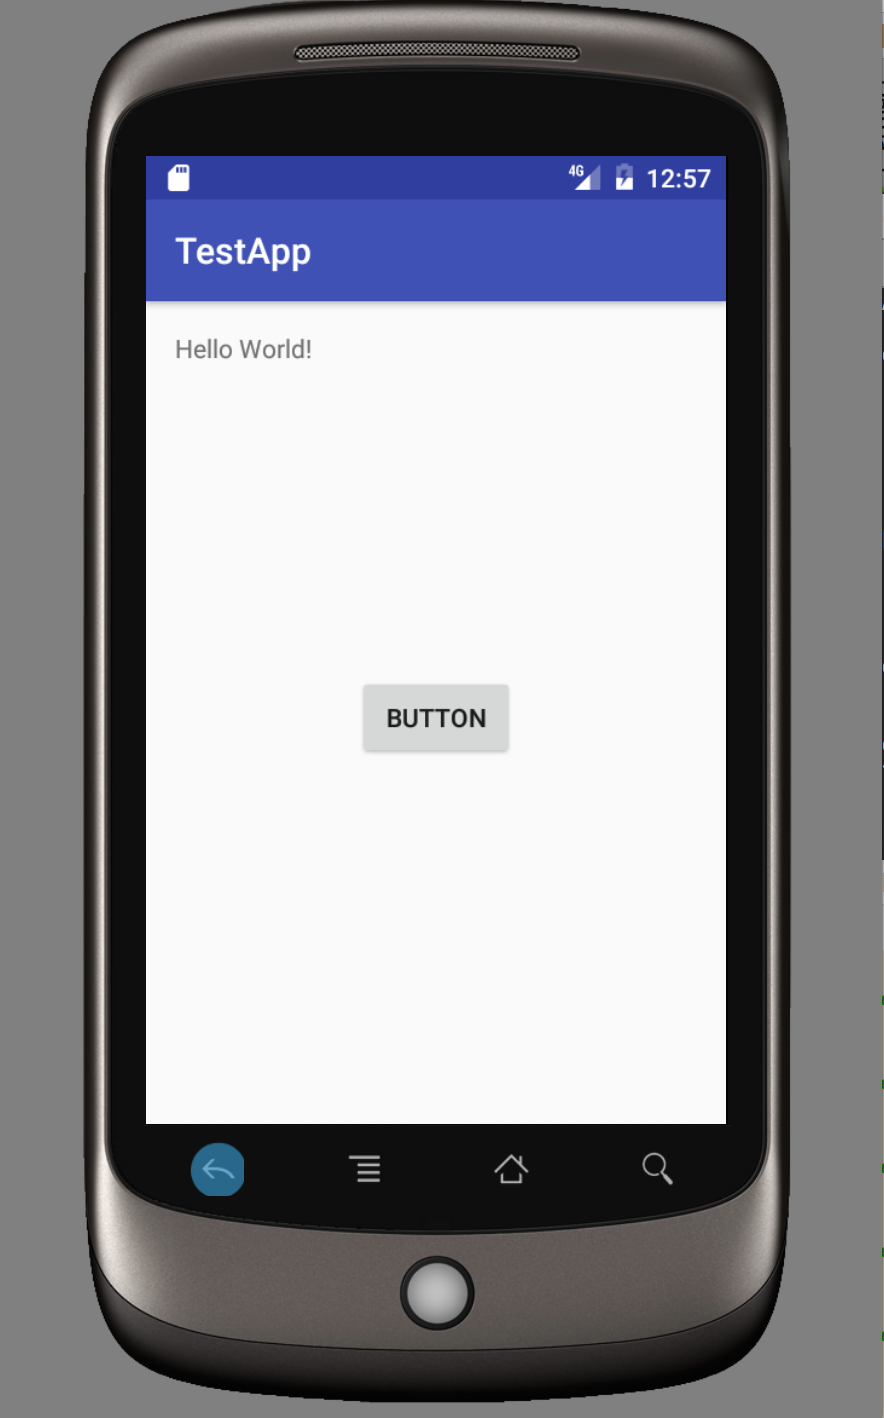
\includegraphics[width=\textwidth]{images/launching_activities_1}
        \caption{The first Activity that is launched}
        \label{fig:launching_activities_1}
    \end{subfigure}
    ~ 
    \begin{subfigure}[b]{0.45\textwidth}
        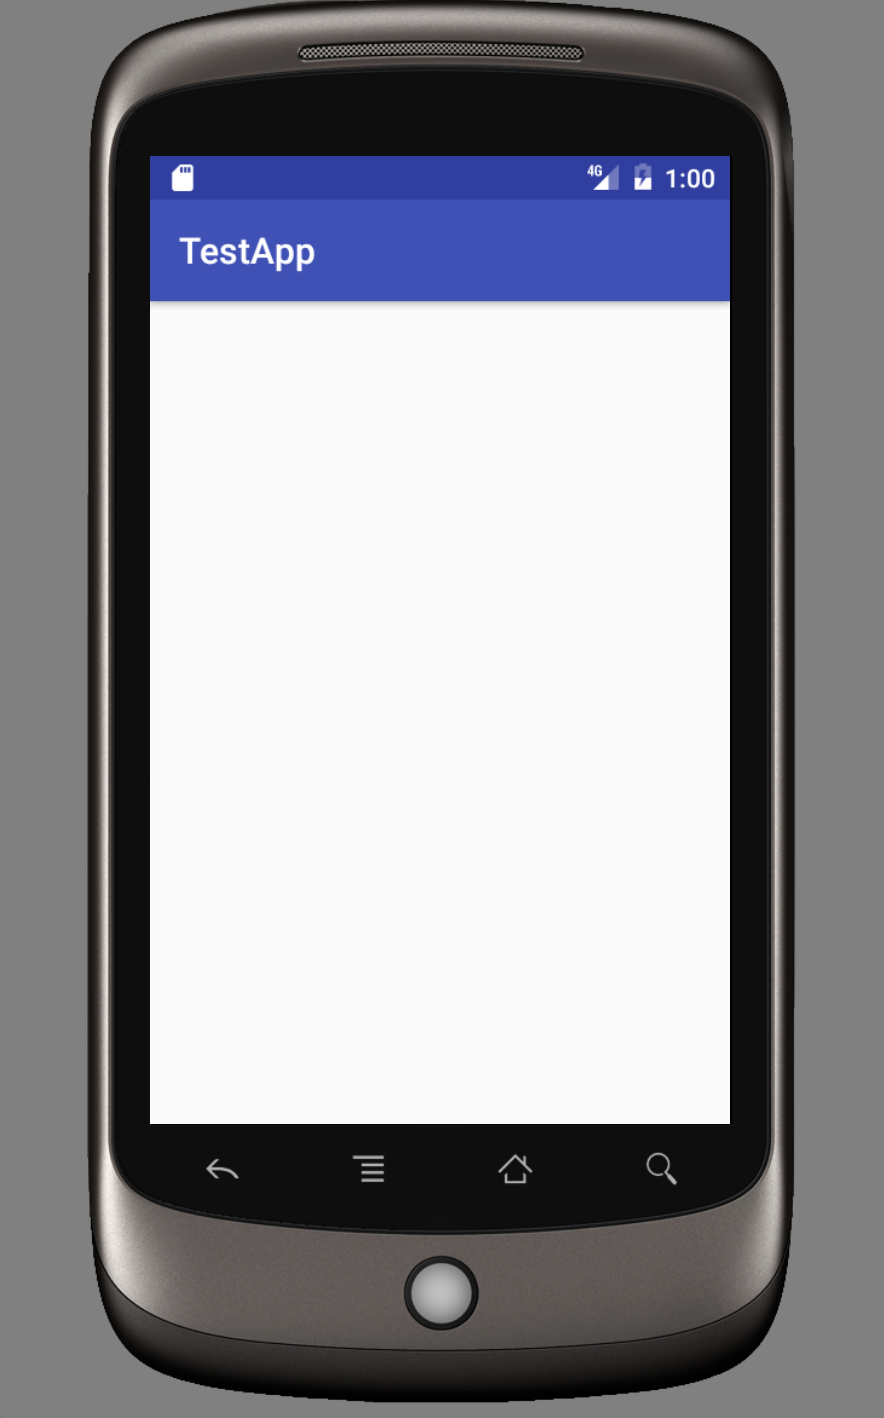
\includegraphics[width=\textwidth]{images/launching_activities_2}
        \caption{The second Acitivty that is launched}
        \label{fig:launching_activities_2}
    \end{subfigure}
\caption{The Activity shown in \ref{fig:launching_activities_1} is displayed first then once the button is clicked the Activity shown in \ref{fig:launching_activities_2} is displayed. Recall that new Activities are placed onto the Activity stack, so the Activity shown in \ref{fig:launching_activities_2} is placed on top of \ref{fig:launching_activities_1}. To navitate back from \ref{fig:launching_activities_2} to \ref{fig:launching_activities_1} you must used the device back button. }
\label{fig:launching_activities}
\end{figure}



%\subsection{Managing Multiple Activities}
%\paragraph{} Rather than creating a new activity for every screen in your app, it make sense to reuse resources when appropriate. For example, if your user is presented with a list of items that can be displayed, you could either have an activity for each item and switch between them after user interaction, or a single activity, designed to display your items consistently, which is reused based on user interaction. Having less activities, but reusing them in a sensible manner can help to stop your app from becoming unmanageable.


%\section{ViewGroups \& Layouts}
%\paragraph{}


\section{Some User Input}
\paragraph{} Remember, views are widgets that have an appearance onscreen. So user input widgets, such as text inputs, can use views just as output does. Let's explore some user input.

\paragraph{} Create a new project and check that it runs properly. Now delete the Hello World TextView so that we have an empty layout to play with.

\paragraph{} Add a ScrollView such as the following to your layout:

\begin{lstlisting}
<ScrollView
        android:layout_width="wrap_content"
        android:layout_height="wrap_content"
        android:id="@+id/scrollView"
        android:layout_centerVertical="true"
        android:layout_alignParentLeft="true"
        android:layout_alignParentStart="true"
        android:layout_marginLeft="42dp"
        android:layout_marginStart="42dp" >

        </ScrollView>
\end{lstlisting}

\paragraph{} Your activity\_main.xml should look similar to the following:

\begin{lstlisting}
<RelativeLayout xmlns:android="http://schemas.android.com/apk/res/android"
    xmlns:tools="http://schemas.android.com/tools" android:layout_width="match_parent"
    android:layout_height="match_parent" android:paddingLeft="@dimen/activity_horizontal_margin"
    android:paddingRight="@dimen/activity_horizontal_margin"
    android:paddingTop="@dimen/activity_vertical_margin"
    android:paddingBottom="@dimen/activity_vertical_margin" tools:context=".MainActivity">

    <ScrollView
        android:layout_width="wrap_content"
        android:layout_height="wrap_content"
        android:id="@+id/scrollView"
        android:layout_centerVertical="true"
        android:layout_alignParentLeft="true"
        android:layout_alignParentStart="true"
        android:layout_marginLeft="42dp"
        android:layout_marginStart="42dp" >
         
    </ScrollView>

</RelativeLayout>
\end{lstlisting}
\paragraph{} Don't worry if everything isn't \emph{exactly} the same. The graphical editor in Android Studio will sometimes try to be helpful and add extra parameters to give you a better layout.

\paragraph{} Now add a LinearLayout as a child of the ScrollView:

\begin{lstlisting}
<LinearLayout
            android:orientation="vertical"
            android:layout_width="fill_parent"
            android:layout_height="fill_parent"
            android:layout_below="@+id/scrollView"
            android:layout_centerHorizontal="true">
</LinearLayout>
\end{lstlisting}

\paragraph{} So you should end up with something like the following:

\begin{lstlisting}
<RelativeLayout xmlns:android="http://schemas.android.com/apk/res/android"
    xmlns:tools="http://schemas.android.com/tools" android:layout_width="match_parent"
    android:layout_height="match_parent" android:paddingLeft="@dimen/activity_horizontal_margin"
    android:paddingRight="@dimen/activity_horizontal_margin"
    android:paddingTop="@dimen/activity_vertical_margin"
    android:paddingBottom="@dimen/activity_vertical_margin" tools:context=".MainActivity">

    <ScrollView
        android:layout_width="wrap_content"
        android:layout_height="wrap_content"
        android:id="@+id/scrollView"
        android:layout_centerVertical="true"
        android:layout_alignParentLeft="true"
        android:layout_alignParentStart="true"
        android:layout_marginLeft="42dp"
        android:layout_marginStart="42dp" >

        <LinearLayout
            android:orientation="vertical"
            android:layout_width="fill_parent"
            android:layout_height="fill_parent"
            android:layout_below="@+id/scrollView"
            android:layout_centerHorizontal="true">

        </LinearLayout>

    </ScrollView>

</RelativeLayout>
\end{lstlisting}

\paragraph{} Neither of these elements, the ScrollView or LinearLayout do much visually. If you run the app now there isn't much to see. But they are containers which will help us to have a nice screen when we add the views in a few moments. For now, notice how the pair of $<$LinearLayout$>$ $<$/LinearLayout$>$ tags are children of, or come between, the $<$ScrollView$>$ $<$/ScrollView$>$ tags. We will deal with Layouts more in next weeks practical but for now just think of them as containers that holds views for you and automatically arrange them for you. All the ScrollView does is make its child view scrollable when the view won't fit on screen. A ScrollView can only have one child, which is our LinearLayout, but the child of the ScrollView can contain multiple further views. Lets try that out.

\paragraph{} Add three TextViews and three EditTexts to your layout so that you have three pairs of TextView then EditText, e.g. TextView, EditView, TextView, EditView, TextView, EditView in a column down the screen. Make sure to give each TextView and EditView an id so that you can reference each individually.Add strings for your TextViews to display so that the first TextView is the user's name, second is email address, and third is password.

\paragraph{} Your layout should now look similar to this:

\begin{lstlisting}
<RelativeLayout xmlns:android="http://schemas.android.com/apk/res/android"
    xmlns:tools="http://schemas.android.com/tools" android:layout_width="match_parent"
    android:layout_height="match_parent" android:paddingLeft="@dimen/activity_horizontal_margin"
    android:paddingRight="@dimen/activity_horizontal_margin"
    android:paddingTop="@dimen/activity_vertical_margin"
    android:paddingBottom="@dimen/activity_vertical_margin" tools:context=".MainActivity">

    <ScrollView
        android:layout_width="wrap_content"
        android:layout_height="wrap_content"
        android:id="@+id/scrollView"
        android:layout_centerVertical="true"
        android:layout_alignParentLeft="true"
        android:layout_alignParentStart="true"
        android:layout_marginLeft="42dp"
        android:layout_marginStart="42dp" >

        <LinearLayout
            android:orientation="vertical"
            android:layout_width="fill_parent"
            android:layout_height="fill_parent"
            android:layout_below="@+id/scrollView"
            android:layout_centerHorizontal="true">

            <TextView
                android:layout_width="wrap_content"
                android:layout_height="wrap_content"
                android:textAppearance="?android:attr/textAppearanceLarge"
                android:text="@string/name"
                android:id="@+id/tv1" />

            <EditText
                android:layout_width="match_parent"
                android:layout_height="wrap_content"
                android:id="@+id/et1"
                 />

            <TextView
                android:layout_width="wrap_content"
                android:layout_height="wrap_content"
                android:textAppearance="?android:attr/textAppearanceLarge"
                android:text="@string/email"
                android:id="@+id/tv2"
                 />

            <EditText
                android:layout_width="match_parent"
                android:layout_height="wrap_content"
                android:id="@+id/et2"
                android:inputType="textEmailAddress"
                 />

            <TextView
                android:layout_width="wrap_content"
                android:layout_height="wrap_content"
                android:textAppearance="?android:attr/textAppearanceLarge"
                android:text="@string/pw"
                android:id="@+id/tv3"
                 />

            <EditText
                android:layout_width="match_parent"
                android:layout_height="wrap_content"
                android:id="@+id/et3"
                android:password="true" />

        </LinearLayout>

    </ScrollView>

</RelativeLayout>

\end{lstlisting}

\paragraph{} Your strings.xml should look similar to this:

\begin{lstlisting}
<?xml version="1.0" encoding="utf-8"?>
<resources>

    <string name="app_name">UserInput</string>
    <string name="hello_world">Hello world!!!!</string>
    <string name="action_settings">Settings</string>
    <string name="name">Name</string>
    <string name="email">Email Address</string>
    <string name="pw">Password</string>

</resources>
\end{lstlisting}

\paragraph{} All other files in your project should be unchanged for now as we have only edited the layour and strings files, so try running your app now. You might want to futher adjust how things look. It is worth taking the time to do that now as this builds your experience of how Android apps work. When you run the app you should be able to input text into the three EditTexts. The password field should hide letters as you type them in. This behaviour is controlled by the following parameter of the EditText: 

\begin{lstlisting}
android:password="true"
\end{lstlisting}

\paragraph{} You should experiment with the other parameters that EditText, and other views have as you explore the Android platform features.

\paragraph{} Now lets consider doing something with the text entered into the EditText fields. Lets add some features to ensure that the name field is limited to a set number of characters in length and only allows names in upper-case. Open MainActivity.java and add the following code to the OnCreate method after the call to setContentView():

\begin{lstlisting}
    EditText nameTxt = (EditText) findViewById(R.id.et1);
    nameTxt.setFilters(new InputFilter[] {
        new InputFilter.LengthFilter(10),
        new InputFilter.AllCaps()
    });
\end{lstlisting}

\paragraph{} All this is doing is creating a variable, called nameTxt, that is associated with the EditText names et1. We have then used some built in classes to set some filters on the EditText, one of which limits the length of input to 10 chars, and the other which enforces upper-case. Run your app and try it out.

\paragraph{} Now lets do somethings a bit more advanced. Lets check the content of the supplied password to see whether it passes muster. For example, lets assume that the supplied password must contain a mixture of letters and numbers. A simple way to do this is to add a button which, when clicked, will take the text in the password field and tell us whether it is valid. So, add a button to your layout, inside the LinearLayout and after the last EditText:

\begin{lstlisting}
<Button
        android:layout_width="wrap_content"
        android:layout_height="wrap_content"
        android:text="@string/go"
        android:id="@+id/btn1"
        android:layout_below="@+id/scrollView"
        android:layout_centerHorizontal="true" />
\end{lstlisting}

\paragraph{} and add its content to the strings.xml e.g.

\begin{lstlisting}
<string name="go">GO!</string>
\end{lstlisting}

\paragraph{} You can run your app now and the button will be visible but it won't do anything because we haven't given it a handler to response to click events. So lets do that, add the following code to the OnCreate method of MainActivity.java after your code that added the input filters to the name field.

\begin{lstlisting}
final EditText pwfield = (EditText) findViewById(R.id.et3);
    Button go_button = (Button) findViewById(R.id.btn1);
    go_button.setOnClickListener(new View.OnClickListener() {
        @Override
        public void onClick(View v) {
            String text = pwfield.getText().toString();

            boolean valid = true;
            boolean hasNumbers = false;
            boolean hasLetters = false;

            for (int i=0; i<text.length(); i++) {
                char x = text.charAt(i);
                if (Character.isDigit(x)){
                    hasNumbers = true;
                }
                else if (Character.isLetter(x)) {
                    hasLetters = true;
                }
                else {
                    valid = false;
                    break;
                }
                if (valid && hasLetters && hasNumbers) {
                    Toast.makeText(getBaseContext(), "Password " + text + " is valid.", Toast.LENGTH_SHORT).show();
                }
                else {
                    Toast.makeText(getBaseContext(), "Password " + text + " is not valid.", Toast.LENGTH_SHORT).show();
                }

            }
        }

    });
\end{lstlisting}

\paragraph{} Most of this is normal Java. You should try to read the code to ensure that you understand exactly what is happening and why.

\paragraph{FURTHER EXERCISE} Try to add a handler for the email field which ensure that the supplied email address is correctly formatted. If you are unsure what constitutes a valid email address then it might be worth finding out more\footnote{\begin{itemize}\item Wikipedia Email Address Page: \url{http://en.wikipedia.org/wiki/Email_address} \item RFC5321 \url{http://tools.ietf.org/html/rfc5321} \item StackOverlfow discussion: \url{http://stackoverflow.com/questions/6119722/how-to-check-edittexts-text-is-email-address-or-not}\end{itemize}}.


\section{Summary}
\paragraph{} In this practical we have 

\begin{itemize}
\item Learnt about Activities
\item Worked with user input
\end{itemize}

